\chapter{Lights} % COMPROBAR TRADUCCIONES

	\section{Runway lights}
		\subsection{Approach lights}
		\paragraph{}Due to the airport characteristics, it is defined as a precision approach runway II and III. According to that ICAO's classification, the starting point in order to design the approach lights is the rule 5.3.4.22. 
		
		The approach lighting system shall consist of a row of lights on the extended centre line of the runway, extending, wherever possible, over a distance of 900 m from the runway threshold. In addition, the system shall have two side rows of lights, extending 270 m from the threshold, and two crossbars, one at 150 m and one at 300 m from the threshold. Furthermore, the lights forming the centre line shall be placed at longitudinal intervals of 30 m with the innermost lights located 30 m from the threshold.
		 
		Moving into the point 5.3.4.24, the lights forming the side rows shall be placed on each side of the centre line, at a longitudinal spacing equal to that of the centre line lights and with the first light located 30 m from the threshold. Where the serviceability level of the approach lights specified as maintenance objectives in 10.5.7 can be demonstrated, lights forming the side rows may be placed on each side of the centre line, at a longitudinal spacing of 60 m with the first light located 60 m from the threshold. The lateral spacing between the innermost lights of the side rows shall be not less than 18 m nor more than 22.5 m, and preferably 18 m, but in any event shall be equal to that of the touchdown zone lights.
		
		Both points 5.3.4.25 and 5.3.4.27 are related to the crossbars. The crossbar provided at 150 m from the threshold shall fill in the gaps between the centre line and side row lights while the one provided at 300m shall extend on both sides of the centre line lights to a distance of 15 m from the centre line.
		
		The next image taken from annex 14 sums up all the points and requirements stated above: 
		
		\begin{figure}[H]
			\centering
			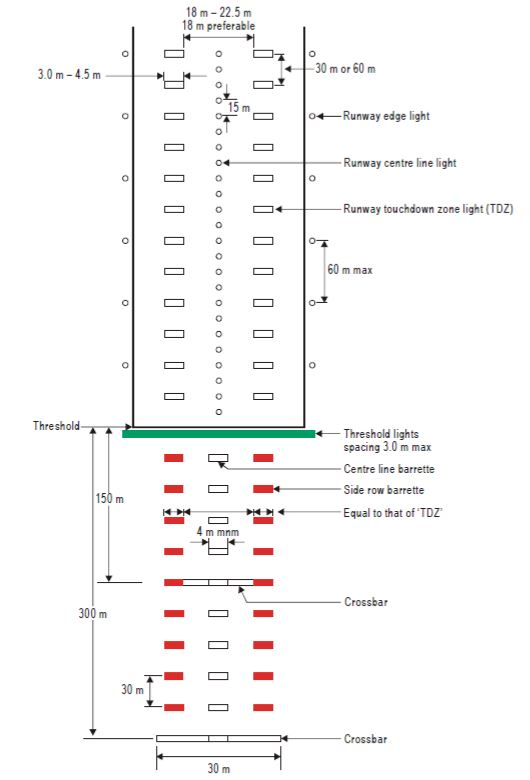
\includegraphics[clip, trim=0cm 0cm 0cm 0cm, width=0.45\textwidth]{./images/Annex14/approachlights}
			\caption{Schematic figure representing the approaching lights.} %nom de la figura
			\label{} %per denotar una referencia
		\end{figure} 
	
		\textbf{\textit{Characteristics}}
		
		According to ICAO, the centre line of a precision approach category II and III lighting system for the first 300 m from the
		threshold shall consist of barrettes showing variable white, except that, where the threshold is displaced 300 m or more, the
		centre line may consist of single light sources showing variable white. 
		
		Since the threshold of both runways is not displaced more than 300m, the centre line will consist of barrettes showing variable white. Those barrettes has to have a minimum length of 4m according to the article number 5.3.4.33.
		
		The side row shall consist of barrettes showing red. The length of a side row barrette and the spacing of its
		lights shall be equal to those of the touchdown zone light barrettes.
		
		\subsection{Approach slope indication systems}
		\paragraph{}There are 4 types of approach slope indication systems: T-VASIS, AT-VASIS, PAPI AND APAPI. Depending on the system chosen, the design may change. In order to ease the maintenance costs and due to its easy design and installation, the system chosen is the PAPI.
		The recommendations and the rules that affect the PAPI and APAPI design range from the statement number 5.3.5.24 until the 5.3.5.41 inclusive.
		
		\textbf{\textit{Description}}
		
		The PAPI system shall consist of a wing bar of four sharp transition multi-lamp units
		equally spaced and the system shall be located on the left side of the runway unless it is physically impracticable to do so. 
		
		The wing bar of a PAPI shall be constructed and arranged in such a manner that a pilot making an approach
		will:
		
		a) When on or close to the approach slope, see the two units nearest the runway as red and the two units farthest from the runway as white.
		
		b) When above the approach slope, see the one unit nearest the runway as red and the three units farthest from the runway as white; and when further above the approach slope, see all the units as white.
		
		c) When below the approach slope, see the three units nearest the runway as red and the unit farthest from the runway as white; and when further below the approach slope, see all the units as red.
		
		\textbf{\textit{Calculations}}
		
		The location of the PAPI system should be the one that brings the highest compatibility with all the other visual and non-visual factors, considering facts such has the vertical distance of the pilot and the antenna of the planes that regularly use the runway. The distance is going to be equal to the medium length between the threshold and the beginning of the landing, adding a corrector factor due to the difference between the vertical length of the pilot eyes and the antenna. This factor can be obtained by multiplying the medium vertical distance between the pilot eyes and the antenna with the cotangent of the approximation angle. 
		
		Considering the landing distance of 400m and making use of the Annex 14, the factor of correction can be obtained considering a landing angle of 3\degree. The value obtained is 53,31m. Thus, the final PAPI location is 453,31m.
		
		In order to state the perpendicular distance between the PAPI and the runway, the following picture taken from ICAO's manual determines that value. 
		
		 \begin{figure}[H]
		 	\centering
		 	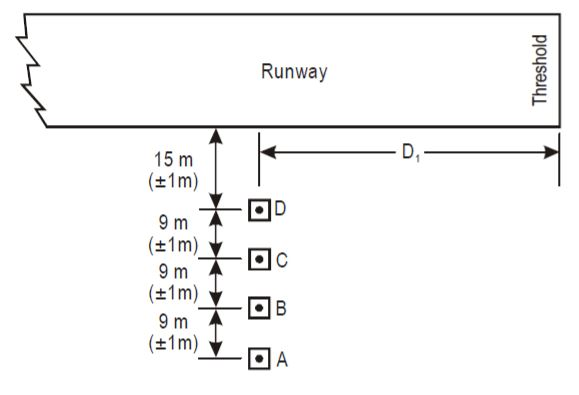
\includegraphics[clip, trim=0cm 0cm 0cm 0cm, width=0.75\textwidth]{./images/Annex14/PAPI}
		 	\caption{Vertical distance between the PAPI and the runway.} %nom de la figura
		 	\label{} %per denotar una referencia
		 \end{figure}
		
		In order to ensure the visibility of the PAPI system, an area empty of obstacles must be defined. The parameters that define this protective surface are gathered in the following table extracted from the Annex 14, chapter 5:
		
		\begin{figure}[H]
			\centering
			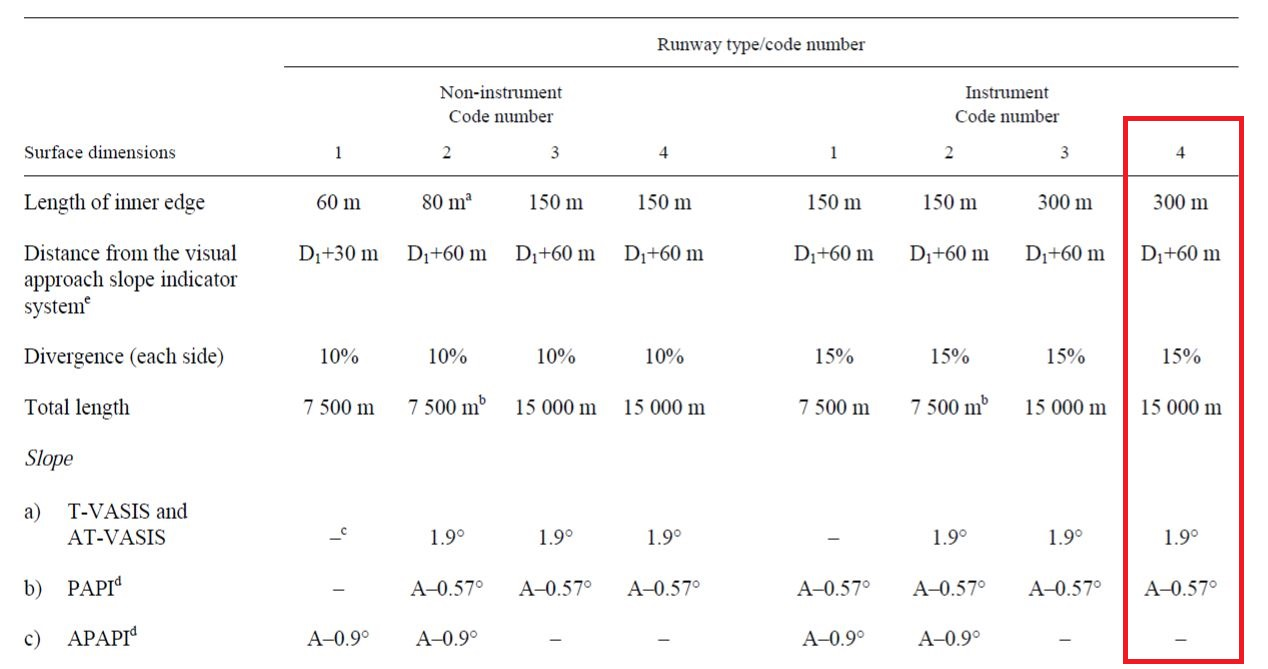
\includegraphics[clip, trim=0cm 0cm 0cm 0cm, width=1\textwidth]{./images/Annex14/SuperficiesPAPI}
			\caption{Dimensions and slopes of the obstacle protection surface.} %nom de la figura
			\label{} %per denotar una referencia
		\end{figure}
		
		The following figure extracted from the ICAO's manual can ease the understanding of the PAPI and its protection surface function:
		
		\begin{figure}[H]
			\centering
			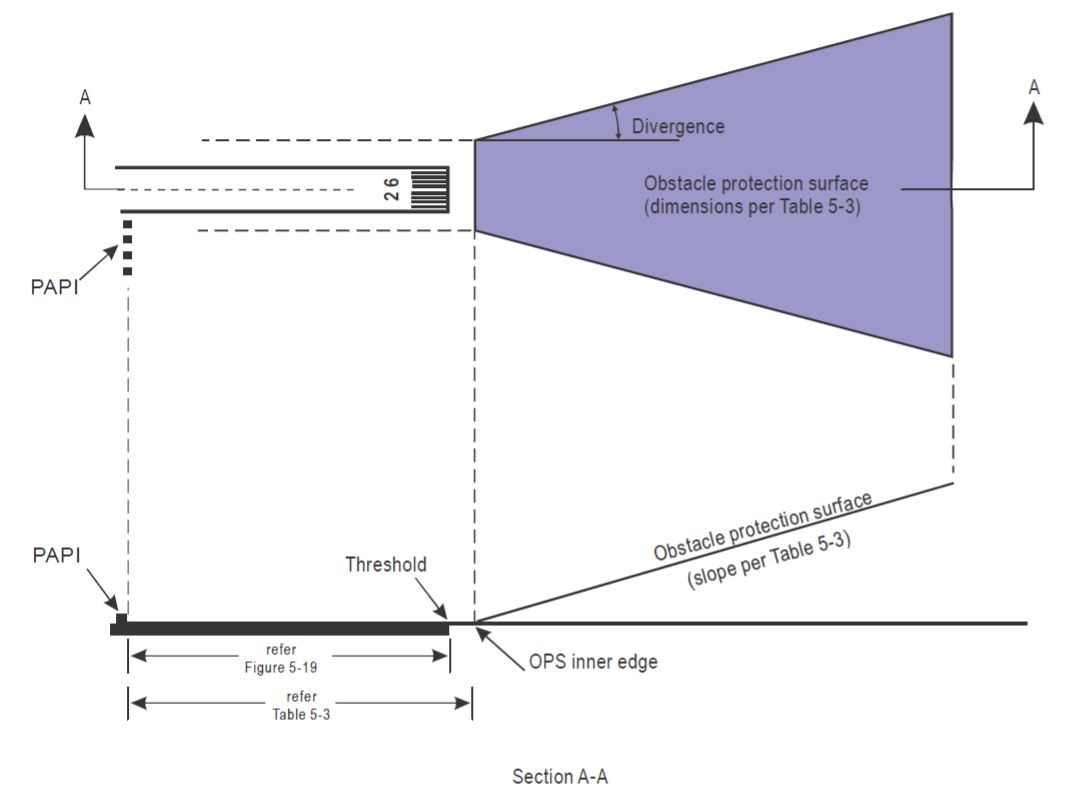
\includegraphics[clip, trim=0cm 0cm 0cm 0cm, width=1\textwidth]{./images/Annex14/PAPIScheme}
			\caption{Protection surface scheme and PAPI positioning.} %nom de la figura
			\label{} %per denotar una referencia
		\end{figure}
		
		\subsection{Runway threshold identification lights}
		\paragraph{}The rules that regulate the runway threshold identification lights can be found on chapter 5.3.8 of the Annex 14. As a conclusion, the following statements define when should the threshold identification lights be included in the airport's installation:
		
		- In a visual approximation runway, when there are no more other reliable visibility aids. 
		
		- The threshold is permanently or temporary displaced from the beginning of the runway.
		
		Due to the fact that non of those requirements are meet, those lights have been discarded.
		 
		\subsection{Runway edge lights}
		\paragraph{}Unlike the last set of lights, the runway edge lights are a must since the airport is expected to work during night time too. 
		
		Runway edge lights shall be placed along the full length of the runway and shall be in two parallel rows equidistant from the centre line. Their distance from the edge should not exceed the 3m. Furthermore, The lights shall be uniformly spaced in rows at intervals of not more than 60 m for an instrument runway. 
		
		Runway edge lights shall be fixed lights showing variable white except 600m before the end of the runway, in this case, may show yellow.
		
		\subsection{Runway threshold and wing bar lights} 
		\paragraph{}Runway threshold will be provided since the runway is equipped with runway edge lights.
		
		\textbf{\textit{Location}}
		
		The threshold lights shall be placed in a row at right angles to the runway axis as near to the extremity of the runway as possible and, in any case, not more than 3 m outside the extreme. Furthermore, due to our approximation category, the lights will be uniformly spaced between the rows of runway edge lights at intervals of not more than 3 m.
		
		The use of wing bars is discarded since any of the runways is considered a visual approaching runway.
		
		\textbf{\textit{Characteristics}}
		
		Runway threshold and wing bar lights shall be fixed unidirectional lights showing green in the direction of approach to the runway.
		
		\subsection{Runway end lights}
		\paragraph{}Following ICAO's legislations, runway end lights shall be provided for a runway equipped with runway edge lights. Their location is on a line as close as possible to the end of the runway, in any case, not more than 3 m outside the end.
		
		\textbf{\textit{Characteristics}}
		
		Runway end lights shall be fixed unidirectional lights showing red in the direction of the runway. The intensity and beam spread of the lights shall be adequate for the conditions of visibility and ambient light in which use of the runway is intended.
		
		The final configuration adding the contribution of the end lights and the threshold lights is the following:
		
		\begin{figure}[H]
			\centering
			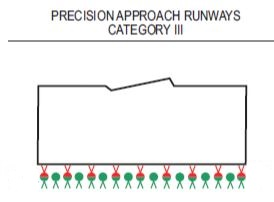
\includegraphics[clip, trim=0cm 0cm 0cm 0cm, width=0.5\textwidth]{./images/Annex14/endlights}
			\caption{Scheme showing the lights placed on the edge of the runway.} %nom de la figura
			\label{} %per denotar una referencia
		\end{figure}
		
		\subsection{Runway centre line lights}
		\paragraph{}According to 5.3.12.11 the airports with precision approach runway of category II or III must provide centre line lights.
		
		 \textbf{\textit{Location}}
		 
		 Runway centre line lights shall be located along the centre line of the runway, except that the lights may be
		 uniformly offset to the same side of the runway centre line by not more than 60cm. The lights shall be located from the threshold to the end at longitudinal spacing of approximately 15m.
		
		\textbf{\textit{Characteristics}}
		
		Runway centre line lights shall be fixed lights showing variable white from the threshold to the point 900 m
		from the runway end; alternate red and variable white from 900 m to 300 m from the runway end; and red from 300 m to the
		runway end, except that for runways less than 1 800 m in length, the alternate red and variable white lights shall extend from
		the midpoint of the runway usable for landing to 300 m from the runway end.
		
		\subsection{Touchdown zone lights}
		\textbf{\textit{Location}}
		
		Touchdown zone lights shall extend from the threshold for a longitudinal distance of 900m and the longitudinal spacing between pairs of barrettes shall be either 30m or 60m.
		
		\textbf{\textit{Characteristics}}
		
		A barrette shall be composed of at least three white unidirectional variable lights with a spacing between the lights of not more than 1,5m. Its length will be higher than 3 and lower than 4,5m in order to successfully follow the recommendation 5.3.13.4.
			
		\subsection{Rapid exit taxiway indicator lights}
		\paragraph{}A set of rapid exit taxiway indicator lights shall be located on the runway on the same side of the runway centre line as the associated rapid exit taxiway. In each set, the lights shall be located 2 m apart and the light nearest to the runway centre line shall be displaced 2 m from the runway centre line. Furthermore, rapid exit taxiway indicator lights shall be fixed unidirectional yellow lights, aligned so as to be visible to the pilot of a landing aeroplane in the direction of approach to the runway. 
		
		The following scheme simplifies the explanation shown above and can also be used to give an example of the application of the rapid exit taxiway indicator lights:
		
		\begin{figure}[H]
			\centering
			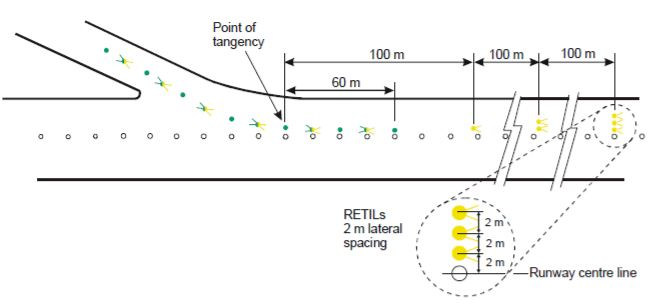
\includegraphics[clip, trim=0cm 0cm 0cm 0cm, width=0.85\textwidth]{./images/Annex14/rapidexittaxiways}
			\caption{Example of rapid exit runway lights.} %nom de la figura
			\label{} %per denotar una referencia
		\end{figure}
	
	\section{Taxiway lights}
		\subsection{Taxiway lights}
		\subsection{Taxiway lights for an exit taxiway}
		\subsection{Taxiway light for a rapid exit taxiway}
		\subsection{Taxiway edge lights}
		\subsection{Stop bar lights}
		\subsection{Intermediate holding point lights}
	
	\section{Apron lights}
		\subsection{Centre line and edge apron lights}
		Due to the fact that many taxiways light interfere with the apron area, such as the article 5.3.22 and the 5.3.17.1, the decision made is to configure the centre line and edge apron lights like in the runways.
	
		\subsection{Projector based apron lighting}
		Due to the fact that the apron is going to be used during night-time, the use of some high power illumination is a must. According to the point 5.3.24.3, the spectral distribution of apron floodlights shall be such that the colours used for aircraft marking connected with routine servicing, and for surface and obstacle marking, can be correctly identified.
		
		Furthermore, even tough it is not a must, some other recommendations will be followed, such as an horizontal luminance of 20lux with a uniformity ratio of not more than 4 to 1; and a vertical luminance of 20lux at a height of 2m above the apron in relevant directions. 
		
		The lights installed on the terminal will follow the orientation shown in the picture below, as it can be seen, noon of them is directly pointing to any pilot.
		
		\begin{figure}[H]
			\centering
			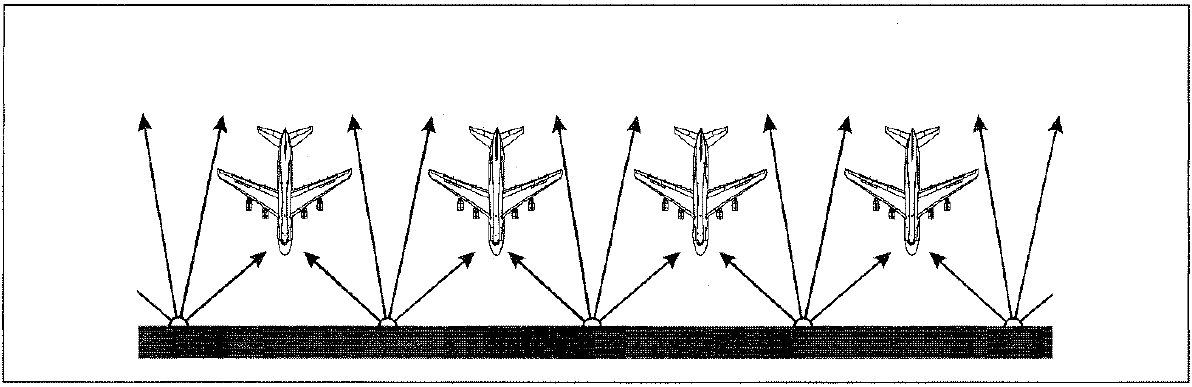
\includegraphics[clip, trim=0.3cm 0.3cm 0.3cm 0.3cm, width=0.95\textwidth]{./images/lights/apronlights}
			\caption{Terminal's fixed projectors and their orientation.} %nom de la figura
			\label{} %per denotar una referencia
		\end{figure}
		
		
		\subsection{Visual guidance system for parking}
		Following the point stated in 5.3.25.1, a visual docking guidance system shall be provided when its intended to indicate, by a visual aid, the precise position of an aircraft stand. 
		
		\textbf{\textit{Characteristics}}
		
		According to ICAO, the azimuth guidance unit and the stopping position indicator shall be located in such a way that there is continuity of guidance between the aircraft stand markings, the aircraft stand manoeuvring guidance lights, if present, and the visual docking guidance system. Furthermore, the system should be able to be shut down by the pilot at any means and should indicate its malfunction in case of it.
		
		In addition, the accuracy of the system should be adequate to the type of air plane and airport.
		
		\underline{\textbf{\textit{Azimuth Guidance Unit}}}
		
		\textbf{\textit{Location}}
		
		According to article 5.3.25.9, the azimuth guidance unit should be located on or close to the extension of the stand line ahead of the aircraft so that its signals are visible from the cockpit and aligned for use at least by the pilot occupying the left seat. 
		
		\textbf{\textit{Characteristics}}
		
		The azimuth guidance unit shall provide unambiguous left/right guidance which enables the pilot to acquire and maintain the lead-in line without over-controlling.
		
		Furthermore, when azimuth guidance is indicated by colour change, green shall be used to identify the centre line and red for deviations from the centre line.
		
		\underline{\textbf{\textit{Stop position indicator}}}
		
		\textbf{\textit{Location}}
		
		The stopping position indicator shall be located in conjunction with, or sufficiently close to, the azimuth guidance unit so that a pilot can observe both the azimuth and stop signals without turning the head. Once more, the stop position indicator should at least be usable for the pilot occupying the left seat.
		
		\textbf{\textit{Characteristics}}
		
		The stopping position indicator shall show the stopping position for the aircraft for which guidance is being provided and shall provide closing rate information to enable the pilot to gradually decelerate the aircraft to a full stop at the intended stopping position.
	